% ------------------------------------------------------------------------------
\section{The PDF Trust Chain \note{1.5pp}}
\label{sec:trust-chain}

What do we mean by the term ``PDF Trust Chain'' in our title?

\subsection{Trust Chains}

The term \emph{Trust Chain} is used in multiple contexts, e.g.,
\emph{digital certificates}: a sequence of certificates signing certificates,
starting with a root certificate;
\emph{supply chain}: a product is no more reliable or secure as its
outsourced components;
\emph{trusted boot}: unless the bootloader is correct and non-malicious,
there can be no possibility of the operating system being the same;
\emph{software stacks}: upper layers are dependent upon lower layers (such as
system libraries) and vulnerabilities at the bottom affect all layers above.

The common idea is that we have layers/components that rely on lower
layers/sub-components/etc for their validity.
And the key lesson being,
{\bf{if a single element of the trust chain 
  is flawed or suborned, then every element ``above'' it
  is no longer capable of being trusted.}}


\subsection{The Trust Chain Inside PDF Parsers}

% In \cref{sec:pdf-challenges}, we elaborated on the challenges of PDF.
% Parsing data-formats has a long history and many solutions ...
% Parsing formal languages also has a long history and many solutions ...
% PDF has aspects of both: this makes PDF challenging.
% But PDF ``parsing'' is not merely a matter of harder [difference of degree]
% but intrinsically more complex [a difference of kind!]:

\begin{figure}[t]
    \centering
    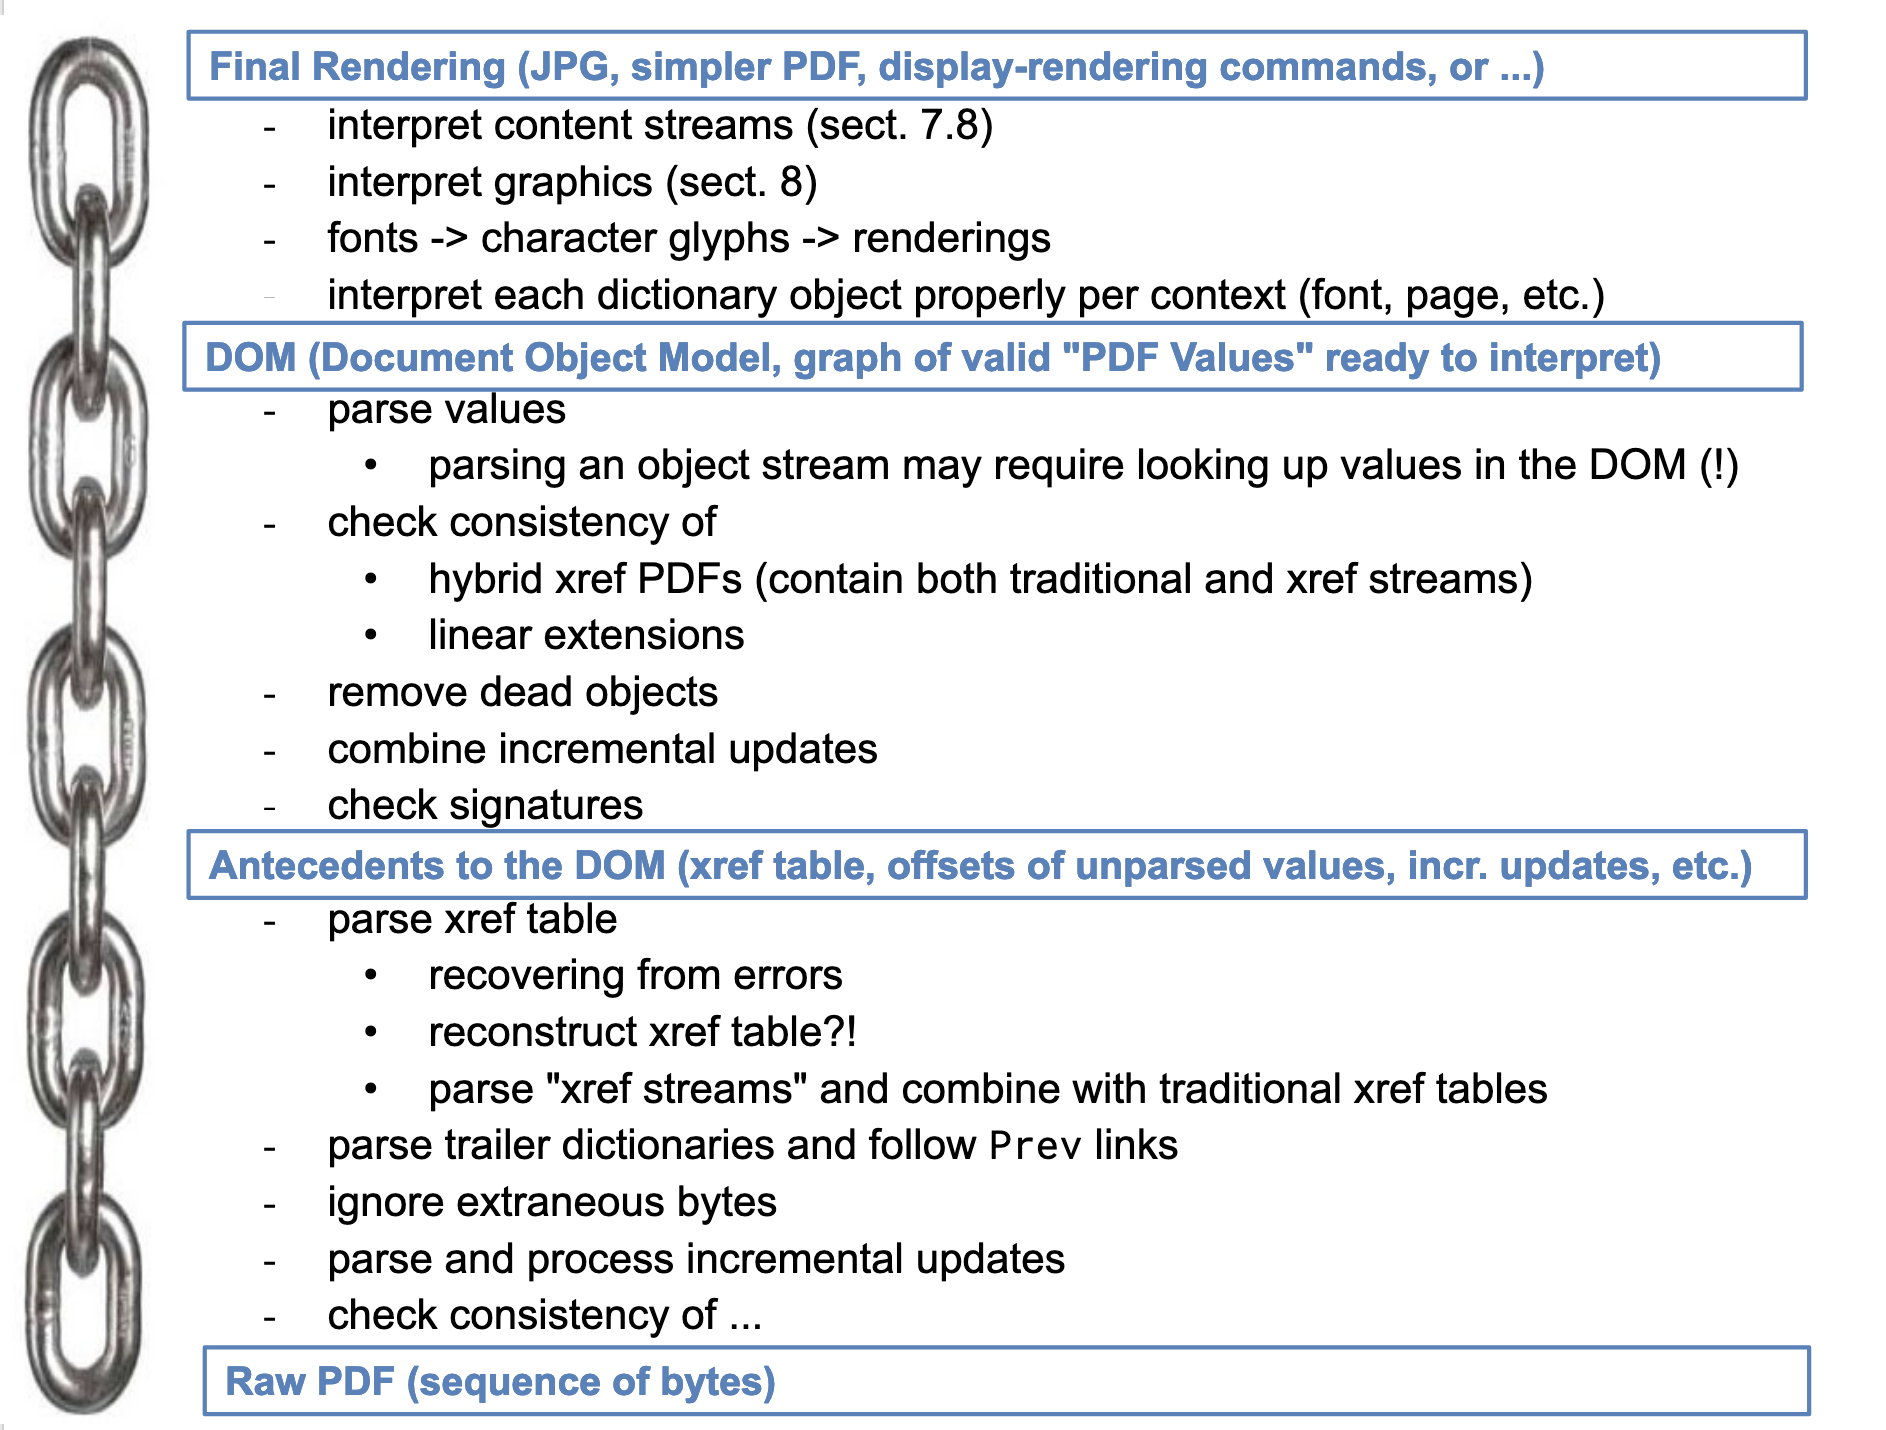
\includegraphics[width=\linewidth]{figures/trustchain-diagram.png}
    \todo{revamp diagram - please add "phase" initiate processing = seek to EOF, locate startxref keyword, etc.}
    \caption{The PDF Trust Chain diagramed.}
    \label{fig:pdf-trust-chain}
\end{figure}

In \cref{sec:pdf-challenges} we touched upon the complexities of parsing
PDF, but to appreciate these, one has to understand the
dependencies and interactions between the \todo{features/aspects/?}.
In \cref{fig:pdf-trust-chain} we attempt to show these diagrammatically.
\todo{explain the [reworked] diagram ...}

% between the ``phases'' of the parsing process.

The attentive reader will note that we have another instance of a \emph{Trust
Chain}.  The later phases of the parsing process are \emph{completely
dependent} upon the earlier phases to properly parse and interpret the PDF
file.

% The PDF "trust chain": higher levels of abstraction depend upon lower levels.
% These structures are not necessarily concrete values--e.g. parsed xref
% table--but they do exist `conceptually'.

We think understanding a PDF parser in terms of this \emph{Trust Chain} is
important:
%
(1) it highlights the presence of the many ``dependent'' parsers (or phases)
in PDF processing.
%
(2) it highlights the importance of ensuring the pre-DOM parsing and
computation (the base of our Trust Chain) is correct and secure.
%
(3) it reminds us that the integrity of the DOM cannot be verified
independently of the lower levels.

\todo{introduce terms such as Pre-DOM}
\todo{say ... regarding our repetitious use of ``parse and compute''}
    
% ------------------------------------------------------------------------------
\section{Pre-DOM Vulnerabilities \note{2.5pp}}
\label{sec:predom-vulnerabilities}

As will become even more apparent, there is a significant amount of
parsing and computation that needs to be done \emph{pre-DOM}.
And given our recent points about the \emph{PDF Trust Chain}
(\cref{sec:trust-chain}),
it should not surprise us that most of the PDF attack vectors
(\cref{sec:pdf-vulnerabilities})
involve some aspect of breaking the \emph{DOM} abstraction.
I.e., they occur at the \emph{pre-DOM} levels.

\todo{notion of cavities [belongs?]}

{\bf{Shadow Attacks}} \todo{...}

{\bf{Schizophrenia}} \todo{...}
\begin{lstlisting}[style=meta]
  - writer errors
  - parser differentials
    - e.g., ignoring xref tables
  - recovering parsers !!
  - blind faith in incremental updates (Shadow Attacks)
\end{lstlisting}

{\bf{Polyglots}} 
\todo{... arising from cavities and permissive implementations and ...}

{\bf{Denial of Service (DOS)}} 
%
\begin{lstlisting}[style=meta]
- [potential recursion many places]
- format may not be well-defined because the recursion is not
    "well-defined"
\end{lstlisting}

{\bf{Others}} \todo{have any others here??}